%    2. Write your answers in section "B" below. Precede answers for all 
%       parts of a question with the command "\question{n}{desc}" where n is
%       the question number and "desc" is a short, one-line description of 
%       the problem. There is no need to restate the problem.
%    3. If a question has multiple parts, precede the answer to part x with the
%       command "\part{x}".
%    4. If a problem asks you to design an algorithm, use the commands
%       \algorithm, \correctness, \runtime to precede your discussion of the 
%       description of the algorithm, its correctness, and its running time, respectively.
%    5. You can include graphics by using the command \includegraphics{FILENAME}
%
\documentclass[11pt]{article}
\usepackage{amsmath,amssymb,amsthm}
\usepackage{graphicx}
\usepackage[margin=1in]{geometry}
\usepackage{fancyhdr}
\usepackage{float}
\newcommand\ceil[1]{\lceil#1\rceil}
\setlength{\parindent}{0pt}
\setlength{\parskip}{5pt plus 1pt}
\setlength{\headheight}{13.6pt}
\newcommand\question[2]{\vspace{.25in}\hrule\textbf{#1}\vspace{.5em}\hrule\vspace{.10in}}
\renewcommand\part[1]{\vspace{.10in}\textbf{(#1)}}
\pagestyle{fancyplain}
\lhead{\textbf{\NAME\ (\UID)}}
\chead{\textbf{Optimization and Online Learning}}
\rhead{CS 6966, \today}
\begin{document}\raggedright

\newcommand\NAME{Jake Pitkin}
\newcommand\UID{u0891770}
\newcommand\HWNUM{2}

\question{Problem 6 - Convexity Basics}

For this problem, let $f$ be a convex function defined over a convex set $K$, and suppose the diameter of $K$ is $1$.

\part{a} Let $x \in K$, and suppose $f(x) = 2$ and $\vert \vert \nabla f(x) \vert \vert = 1$. Give a lower bound on min$_{z \in K}$ $f(z)$.

\fbox{ \parbox{1\linewidth}{

} }

\part{b} Let $x^*$ be the minimizer of $f$ over $K$ (suppose it is unique), and let $x$ be any other point. The intuition behind gradient descent is that the vector: $- \nabla f(x)$ points \textit{towards} $x^*$. Prove that this is indeed true, in the sense that $\langle \nabla f(x), x - x^* \rangle \geq 0$ (i.e., the negative gradient makes an acute angle with the line to the optimum).

\fbox{ \parbox{1\linewidth}{

} }

\part{c} Suppose now that the function $f$ is \textit{strictly convex} i.e., $f(\lambda x + (1 - \lambda) y) < \lambda f(x) + (1 - \lambda) f(y)$ (strictly), for all $x \neq y$, and $0 < \lambda < 1$. Prove that all the \textit{maximizers} of $f$ over $K$ lie on the boundary of $K$. [\textit{Hint:} You many want to use the definition that a point $x$ is not on the boundary iff there exists points $y, z \in K$ such that $x = (y + 2)/2$.]

\fbox{ \parbox{1\linewidth}{

} }

\question{Problem 7 - Gradient Descent Basics}

\part{a} Give an example of a function defined over $\mathbb{R}$, for which for \textit{any} step-size $\eta > 0$ (no matter how small), gradient descent with step-size $\eta$ oscillates around the optimum point (i.e., never gets to distance $< \eta/4$ to it), for some starting point $x \in \mathbb{R}$.

\fbox{ \parbox{1\linewidth}{
Consider the absolute value function $g(x) = |x|$ defined over $\mathbb{R}$.

\begin{figure}[H]
  \centerline{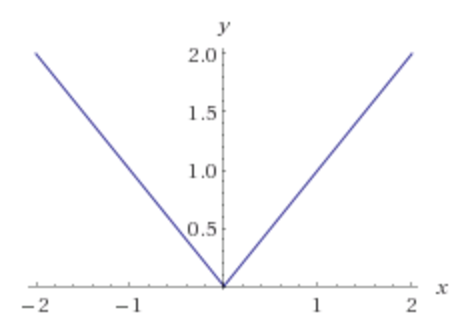
\includegraphics[width=0.4\linewidth]{abs.png}}
\end{figure}

The absolute value function is convex but it is not smooth. It is not differentiable as the derivative at $x = 0$ is not defined. For any arbitrarily small step-size $\eta$, we can find a starting point $x \in \mathbb{R}$ such that gradient descent will oscillate around the optimum point (never getting to distance $< \eta /4$ to it). \\

Each iteration gradient descent takes a step in the direction of the negative gradient at the current point, with a step-size of $\eta$.

$$\mathbf{w}^{(t + 1)} = \mathbf{w}^{(t)} - \eta \nabla g(\mathbf{w}^{(t)})$$

The $\nabla g(x)$ is defined as

$$
\nabla g(x) = \left\{
        \begin{array}{ll}
            -1 & \quad x < 0 \\
            undefined & \quad x = 0 \\
            1 & \quad x > 0
        \end{array}
    \right.
$$

As such, we can see at each iteration of gradient descent we will take a $ \eta$ sized step from the current point. This step will be in the positive direction if $x$ is negative and vice-versa. Thus, regardless of how small $\eta$ is, we can easily arrive at a situation where gradient descent will oscillate around the optimum point found at the origin.

} }

\part{b} Consider the function $f(x, y) = x^2 + \frac{y^2}{4}$, and suppose we run gradient descent with starting point $(1, 1)$, and $\eta = 1/4$. Do we get arbitrarily close to the minimum? Experimentally, find the \textit{threshold} for $\eta$, beyond which the gradient descent starts to oscillate.

\fbox{ \parbox{1\linewidth}{
Given the function $f(x, y) = x^2 + \frac{y^2}{4}$ with a starting point of $\mathbf{w}^{(1)} = (1, 1)$ and $\eta = 1/4$ we get arbitrarily close to the minimum. The minimum of $f(x, y)$ is 0 when $\mathbf{w} = (0, 0)$. To explore this gradient descent scenario, I wrote a program to calculate $\mathbf{w}^{(t)}$ and defined arbitrarily close to being within $0.0001$ of the minimum. I found after 39 steps that $\mathbf{w}^{(39)} = (3.6379\mathrm{e}{-12}, 0.0063)$ and $f(x, y) = 9.7848\mathrm{e}{-06}$. Given enough iterations, the gradient descent found the optimum point. \\

Using a program, I found the threshold for $\eta$. I found the gradient descent starts to oscillate when $\eta \geq 1$. When $\eta = 1$, the behavior is interesting. The $x$ component of $\mathbf{w}^{(t)}$ alternates between the values $1$ and $-1$ and the $y$ component converges to $0$. As such, $f(x, y)$ oscillates between $-1$ and $1$.
} }

\part{c} Why is the behavior similar to that in part (a) (oscillation for every $\eta$) not happening in part (b)?

\fbox{ \parbox{1\linewidth}{
In part (a) we observed that the absolute value function $g(x) = |x|$ oscillates around the optimum point despite choosing an arbitrarily small step-size $\eta$. In part (b) we concluded that $f(x, y) = x^2 + \frac{y^2}{4}$ with reach the optimum point given a step-size $\eta < 1$. \\

If we consider the gradient of $f(x, y)$ which is defined as 

$$\nabla f(x, y) = (2x, \frac{y}{2})$$

and the update for each iteration of gradient descent

$$\mathbf{w}^{(t + 1)} = \mathbf{w}^{(t)} - \eta \nabla f(\mathbf{w}^{(t)})$$

We can observe that $\mathbf{w}^{(t + 1)}$ is dependent on the value of $x_t$, $y_t$, and a fixed $\eta$. As $x_t$ and $y_t$ get closer to 0, the update "size" at each iteration decreases (since $\vert \vert \nabla f(x, y) \vert \vert$ decreases). This was not the case with $g(x)$, as the direction of the update is dependent on $x$ but the "size" of the update is only dependent on $\eta$. Thus, with a reasonably small $\eta$, $f(x, y)$ will reach the optimum point.

} }

\question{Problem 8 - Stochastic Gradient Descent}

Suppose we have points $(a_1, b_1), (a_2, b_2), ... , (a_n, b_n)$ in the plane and suppose that $\vert a_i \vert \leq 1$, and $\vert b_i \vert \leq 1$ for all $i$. Let $f(x, y) = \frac{1}{n} \sum_{i = 1}^n f_i(x, y)$, where $f_i(x, y) = (x - a_i)^2 + (y - b_i)^2$.

\part{a} What is the point $(x , y)$ that minimizes $f(x, y)$?

\fbox{ \parbox{1\linewidth}{

} }

\part{b} Suppose we perform gradient descent (on $f$) with step size $0 < \eta < 1$. Give the geometric interpretation for one iteration.

\fbox{ \parbox{1\linewidth}{

} }

\part{c} Now suppose we perform stochastic gradient descent with fixed step-size $0 < \eta < 1$, and by picking $i$ at random in $\{1, ... , n\}$, and moving along the gradient of $f_i$ (as in SGD seen in class). After $T$ steps, for $T$ large enough, can we say that we get arbitrarily close to the optimum? (Provide a clear explanation). [\textit{Hint:} Remember $\eta$ is fixed.]

\fbox{ \parbox{1\linewidth}{

} }

\part{d} Pick $n = 100$ random points in $[-1, 1]^2$ (uniformly), and run SGD for fixed $\eta = 1/2$, as above. Write down what the distance to optimum is, after $T = 10$, $T = 100$, and $T = 1,000$ iterations (if you want to be careful, you should average over 5 random choices for the initialization). Now consider dropping step size $\eta_t = 1/t$, and write down the result for $T$ as above.

\fbox{ \parbox{1\linewidth}{

} }

\question{Problem 9 - Numeric Accuracy in MW Updates}

Consider the randomized experts setting we saw in class (we maintain a distribution over experts at each time, and the loss of the algorithm at that time is the expected loss over the distribution). Consider the simple setting where the experts predict $0/1$, and the loss is either $0$ or $1$ for each expert. We saw how to update the probabilities (multiply by $e^{-\eta}$ if an expert makes a mistake, keep unchanged otherwise, and renormalize). One of the common problems here is that numeric errors in such computations tend to compound if not done carefully.

\part{a} Consider one simple suggestion: say we zero out weights that are ``too small'', specifically, suppose we set $q_i^{(i)} = 0$ if $q_i^{(i)} /$ max$_j \ q_t^{(i)} < \epsilon$, for some precision parameter ϵϵ (such changes frequently occur due to roundoff). Other than this, suppose that the $q_t^{(i)}$ are updated accurately. Prove that in this case, we cannot hope to achieve any non-trivial regret bound. Specifically, for large enough $T$, the algorithm can have error $T(1 - o(1))$, while the best expert may have error $o(T)$. [Hint: in this case, we are ``losing'' all information about an expert.]

\part{b} A simple way to avoid this (in this setting) is to avoid storing probabilities, but instead maintaining only the number of mistakes $m_t^{(i)}$. Prove how this suffices to recover the probabilities $p_t^{(i)}$ (assuming infinite precision arithmetic).

\fbox{ \parbox{1\linewidth}{

} }

\part{c}  Suppose we use the idea in part (b) to construct a distribution $q_t$ that differs from $p_t$ by $< \epsilon$ in the $\ell_1$ norm, i.e., 
$\sum_i \vert p_t^{(i)} - q_t^{(i)} \vert < \epsilon$. Then, assuming we construct such a $q_t$ at time $t$ to sample, show that the expected number of mistakes of the algorithm is bounded by $(1 + \eta)$ min$_i \ m_T^{(i)} + O(\log N/\eta) + \epsilon T$.

\fbox{ \parbox{1\linewidth}{

} }

\part{d} The bound above is not great if there is an expert who makes very small number of mistakes (compared to $T$). Noting that we are dealing with binary predictions, can you come up with a way to run the algorithm, so as to obtain a mistake bound of $(1 + \eta + 2 \epsilon)$ min$_i \ m_T^{(i)} + O(\log N/\eta)$?

\fbox{ \parbox{1\linewidth}{

} }

\end{document}